\chapter{Metodologia}
\label{cap:metodologia}


O presente trabalho desenvolveu um sistema para a correção automatizada de provas discursivas. Esse sistema utiliza técnicas avançadas de inteligência artificial, como \textit{Large Language Models} (LLM) e \textit{Retrieval-Augmented Generation} (RAG), permitindo que as avaliações sejam corrigidas de forma rápida, precisa e objetiva. Assim, o processo de avaliação se torna mais eficiente, beneficiando tanto professores quanto alunos.

Este capítulo apresenta o detalhamento do desenvolvimento do sistema implementado, que é dividido em três subprocessos principais: a configuração da prova, a correção geral da prova e a correção específica das respostas que exigem intervenção adicional. Cada subprocesso é explicado detalhadamente, utilizando fluxogramas para ilustrar os passos realizados. A seguir, são apresentados os fluxogramas que ilustram cada um dos subprocessos mencionados (Figuras
\autoref{fig:fluxo-configuracao},
\autoref{fig:fluxo-correcao-prova} e
\autoref{fig:fluxo-correcao-pergunta}).

\begin{figure}[H]
    \centering
    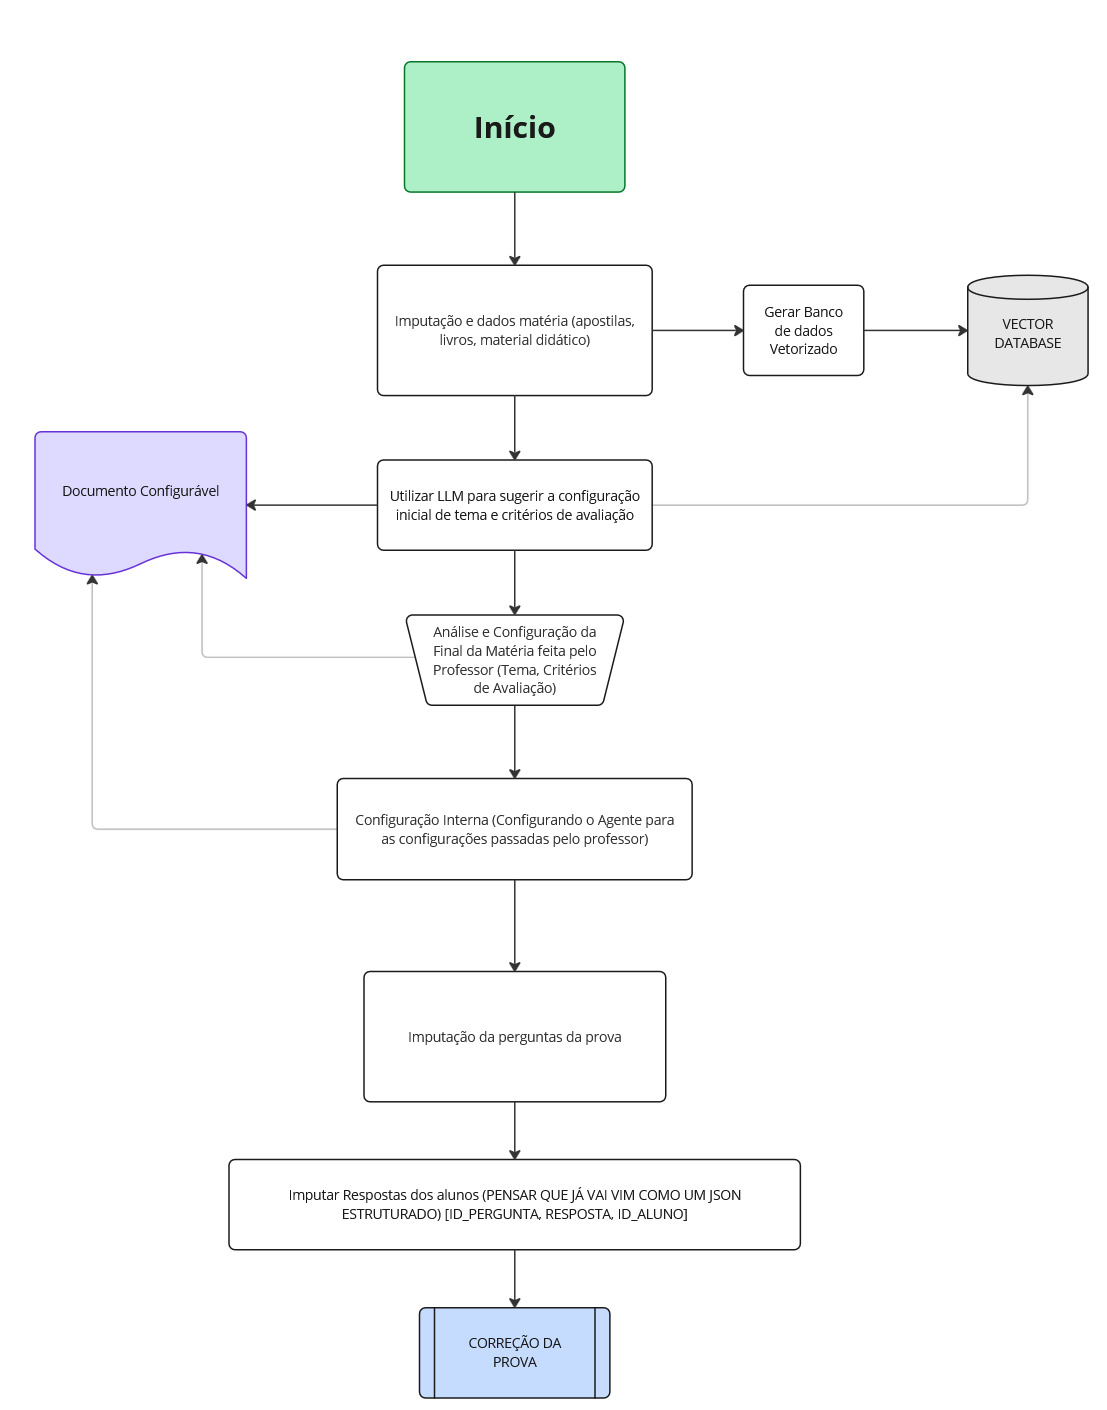
\includegraphics[width=\textwidth]{media/fluxo-configuracao.jpg}
    \caption{Fluxograma do subprocesso de configuração da prova}
    \label{fig:fluxo-configuracao}
\end{figure}

\begin{figure}[H]
    \centering
    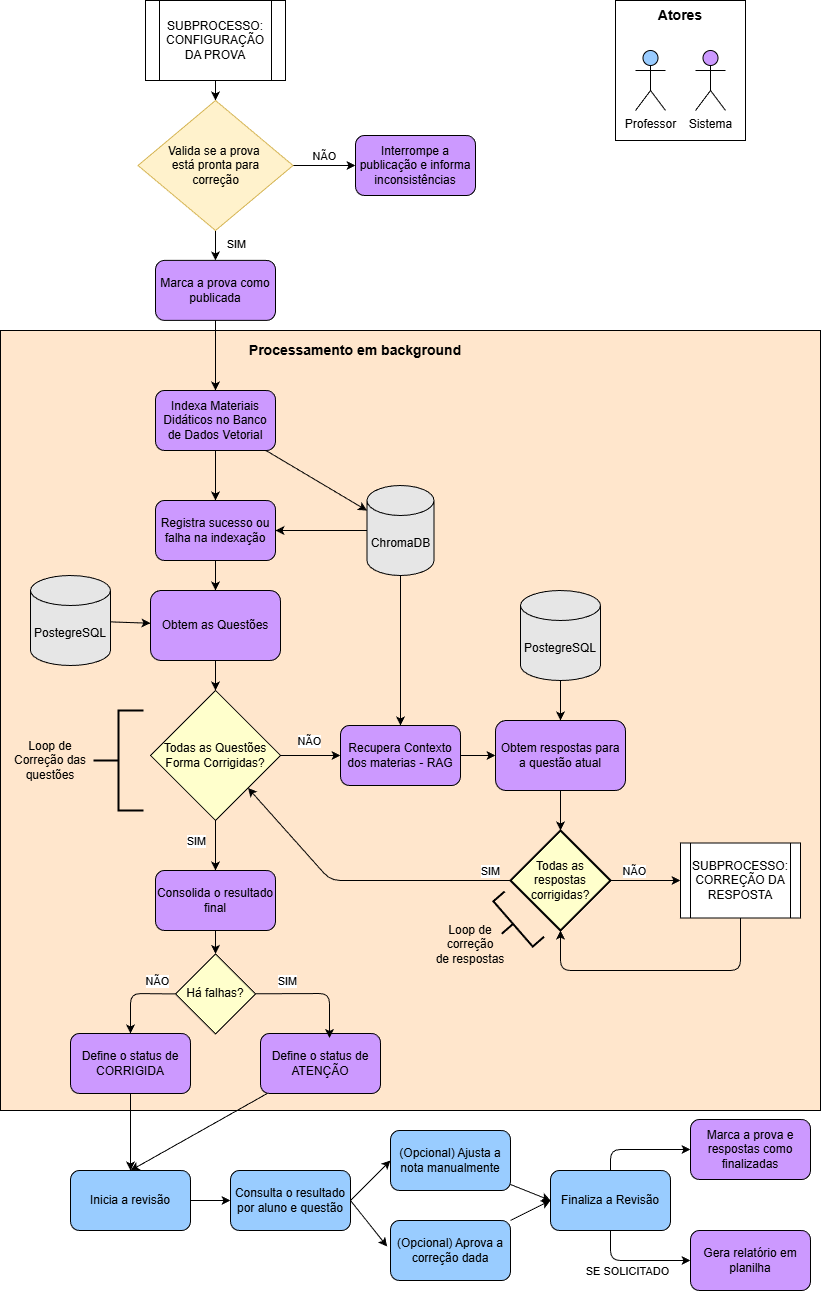
\includegraphics[width=\textwidth]{media/fluxo-correcao-prova.jpg}
    \caption{Fluxograma do subprocesso de correção da prova, incluindo revisão docente antes da consolidação das notas finais}
    \label{fig:fluxo-correcao-prova}
\end{figure}

\begin{figure}[H]
    \centering
    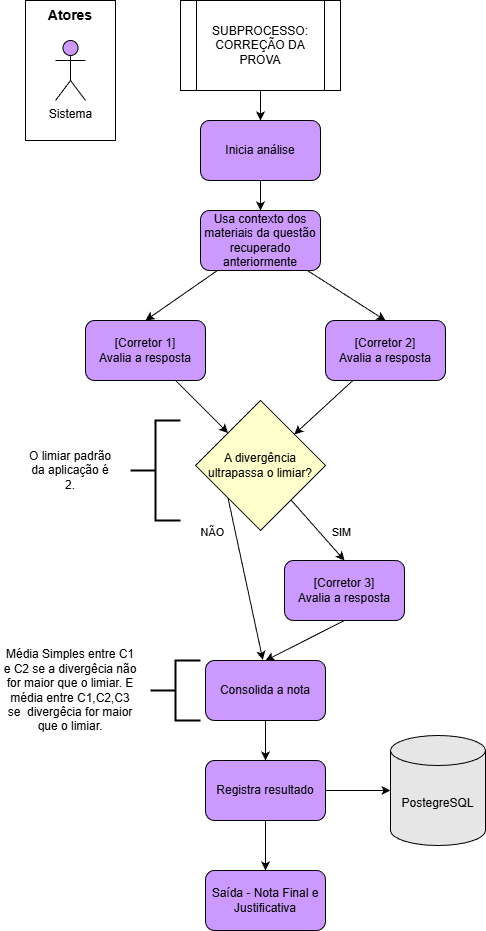
\includegraphics[width=\textwidth]{media/fluxo-correcao-pergunta.jpg}
    \caption{Fluxograma do subprocesso de correção da resposta, com acionamento condicional do Corretor 3 por limiar de divergência}
    \label{fig:fluxo-correcao-pergunta}
\end{figure}

No fluxo da \autoref{fig:fluxo-correcao-prova}, a revisão do professor ocorre após a correção automatizada e a persistência dos resultados no banco de dados, e antes da consolidação/finalização das notas. Já no fluxo da \autoref{fig:fluxo-correcao-pergunta}, o Corretor 3 atua apenas quando a divergência entre o Corretor 1 e o Corretor 2 ultrapassa o limiar configurado, mantendo o caminho condicional de arbitragem alinhado à implementação.

\section{Tipo de Pesquisa}

Este trabalho caracteriza-se como uma pesquisa aplicada, pois desenvolveu um sistema para correção automatizada de provas, visando solucionar um problema prático no contexto educacional. Quanto aos objetivos, classifica-se como uma pesquisa exploratória, já que analisou a viabilidade de implementação de técnicas de inteligência artificial, como LLM e RAG, no processo de correção de avaliações.

\section{Processo de Correção de Prova}

Esta seção descreve o funcionamento do sistema conforme implementado, tomando como referência os fluxos apresentados nas Figuras
\autoref{fig:fluxo-configuracao},
\autoref{fig:fluxo-correcao-prova} e
\autoref{fig:fluxo-correcao-pergunta}.

\subsection{Subprocesso de Configuração da Prova}

O subprocesso de configuração corresponde às etapas realizadas pelo professor antes da publicação da prova (\textit{status} de rascunho). Inicialmente, são definidos metadados gerais (por exemplo, título, descrição e turma), e os materiais didáticos são anexados (principalmente arquivos PDF). Esses anexos são armazenados pela aplicação e registrados no banco de dados relacional, permanecendo indisponíveis para busca semântica até o momento de publicação.

Em seguida, o professor associa critérios de avaliação à prova, definindo pesos e parâmetros de pontuação. Quando necessário, podem ser realizados ajustes específicos por questão, de modo que diferentes questões utilizem variações de rubrica dentro de uma mesma prova. Após essa configuração, as questões são cadastradas com seus enunciados, pontuação e ordem.

Por fim, as respostas discursivas dos alunos são inseridas e persistidas, vinculadas às respectivas questões. Ao publicar a prova, o sistema valida se ela está apta a iniciar o processamento (por exemplo, se permanece em rascunho e se possui questões e respostas registradas). Caso a validação falhe, a publicação é interrompida e as inconsistências são informadas.

\subsection{Subprocesso de Correção da Prova (background e revisão docente)}

Uma vez publicada, a prova dispara um processamento assíncrono em \textit{background}. Esse processamento possui duas responsabilidades principais.

Primeiro, o sistema prepara os materiais didáticos anexados para consulta por similaridade semântica, o que inclui carregar os PDFs, segmentar seu conteúdo em trechos e indexá-los em uma base vetorial. O resultado desse preparo é registrado como sucesso ou falha, o que subsidia a atribuição de um \textit{status} de atenção quando o processamento não se conclui adequadamente.

Segundo, o sistema percorre as questões da prova e executa a correção das respostas discursivas. Para cada questão, o sistema recupera, uma única vez, trechos relevantes dos materiais didáticos utilizando o enunciado como consulta. O contexto recuperado é então reutilizado na correção de todas as respostas associadas àquela questão, reduzindo repetição de consultas e mantendo consistência de referência por questão.

Ao término do processamento, os resultados são consolidados e persistidos, e a prova é marcada com um \textit{status} compatível com o sucesso do fluxo (por exemplo, corrigida quando não há falhas relevantes, ou atenção quando há falhas que exigem intervenção). Em seguida, o professor pode revisar os resultados por aluno e por questão, aprovar respostas e, quando necessário, ajustar manualmente a nota. Ao finalizar a revisão, o sistema registra a finalização da prova e, opcionalmente, disponibiliza um relatório em planilha com a consolidação das notas.

\subsection{Subprocesso de Correção da Resposta (workflow de avaliação)}

O subprocesso de correção da resposta (\autoref{fig:fluxo-correcao-pergunta}) utiliza (i) o texto da resposta do aluno, (ii) a rubrica definida para a questão (critérios, pesos e limites de pontuação) e (iii) o contexto dos materiais didáticos recuperado previamente para a questão.

Inicialmente, dois agentes corretores independentes (Corretor 1 e Corretor 2) avaliam a resposta, produzindo notas e justificativas sem comunicação entre si. Em seguida, o sistema verifica se a divergência entre as avaliações ultrapassa um limiar configurado. Quando a divergência é baixa, a nota final é consolidada diretamente a partir das duas avaliações. Quando a divergência ultrapassa o limiar, um terceiro agente (árbitro) é acionado para uma avaliação adicional.

Ao final, a nota é consolidada por uma regra de consenso e o resultado é persistido, incluindo a nota final e as justificativas associadas. Esse registro alimenta tanto a etapa de consolidação da prova quanto a etapa posterior de revisão docente.

\section{Ferramentas e Tecnologias Utilizadas}

Para o desenvolvimento e a implementação do sistema proposto, foram empregadas ferramentas e tecnologias que atendem aos requisitos de integração com modelos de linguagem, persistência de dados, recuperação de contexto por similaridade semântica e disponibilização do sistema por meio de uma API. A seguir, apresentam-se as principais tecnologias utilizadas e suas respectivas finalidades no contexto do projeto.

\subsection{Python}
O sistema foi implementado em Python, em função da maturidade do ecossistema para desenvolvimento de aplicações web, integração com bibliotecas de inteligência artificial e suporte a ferramentas de persistência e processamento de dados \cite{python_docs_2026}.

\subsection{FastAPI}
O backend foi desenvolvido com o \textit{framework} FastAPI, utilizado para a implementação de uma API REST, organização de rotas e tratamento de requisições relacionadas às etapas de configuração, correção e revisão docente. Para execução em ambiente de produção, a aplicação é servida com \textit{workers} assíncronos (Gunicorn/Uvicorn), favorecendo concorrência e escalabilidade \cite{fastapi_docs_2026,gunicorn_docs_2026,uvicorn_docs_2026}.

\subsection{Orquestração do fluxo com LangGraph}
O fluxo de correção foi estruturado como um grafo de estados, empregando LangGraph para definir nós de execução (recuperação de contexto, correção independente, verificação de divergência, acionamento condicional do terceiro corretor e consolidação do resultado). Essa abordagem permite controlar o encadeamento das etapas e tornar o processo reprodutível e rastreável \cite{langgraph_docs_2026}.

\subsection{Agentes corretores com DSPy e LiteLLM}
Os agentes de correção foram implementados com DSPy, adotando chamadas a modelos de linguagem por meio de uma camada de compatibilidade (LiteLLM). Essa combinação possibilita parametrizar modelos e provedores, manter configuração centralizada e aplicar cache quando aplicável, reduzindo variabilidade operacional e custo computacional \cite{dspy_docs_2026,litellm_docs_2026}.

\subsection{Integração com LLMs e provedores de \textit{embeddings} (LangChain)}
Para padronizar integrações com provedores de modelos e de \textit{embeddings}, foram utilizadas bibliotecas do ecossistema LangChain. No sistema, essa camada é empregada tanto para instanciar modelos de chat (conforme o provedor configurado) quanto para gerar \textit{embeddings} utilizados no processo de recuperação de contexto \cite{langchain_docs_2026}.

\subsection{Recuperação de contexto e armazenamento vetorial (ChromaDB)}
O armazenamento vetorial e a recuperação por similaridade foram realizados com ChromaDB, utilizado como \textit{vector store} persistente. O banco vetorial armazena representações vetoriais dos materiais didáticos e permite consultas para obtenção de trechos relevantes, compondo o contexto adicional necessário à estratégia de \textit{Retrieval-Augmented Generation} (RAG) \cite{chromadb_docs_2026}.

\subsection{Persistência relacional e migrações (PostgreSQL, SQLAlchemy e Alembic)}
Os dados estruturados do sistema (usuários, turmas, provas, questões, respostas, critérios e resultados) são persistidos em banco de dados relacional PostgreSQL. Para a camada de acesso a dados, utiliza-se SQLAlchemy, enquanto Alembic é empregado para versionamento e execução de migrações, assegurando reprodutibilidade do esquema entre ambientes \cite{postgresql_docs_2026,sqlalchemy_docs_2026,alembic_docs_2026}.

\subsection{Conteinerização (Docker e Docker Compose)}
O ambiente de execução foi padronizado por meio de Docker e Docker Compose, viabilizando a composição de serviços (API, banco de dados relacional e serviços auxiliares) e reduzindo diferenças de configuração entre execução local e implantação \cite{docker_docs_2026,docker_compose_docs_2026}.

\subsection{Ollama e Streamlit (apoio a desenvolvimento e inspeção)}
Quando configurado, o Ollama é utilizado como provedor local para modelos e/ou \textit{embeddings}, favorecendo experimentação sem dependência exclusiva de serviços externos. Além disso, uma aplicação auxiliar em Streamlit é utilizada para fins de observabilidade e inspeção do pipeline de correção durante o desenvolvimento \cite{ollama_docs_2026,streamlit_docs_2026}.

\subsection{JSON (\textit{JavaScript Object Notation})}
O formato JSON é empregado na padronização e transmissão de informações entre componentes do sistema, como questões, respostas e identificadores. Essa escolha favorece interoperabilidade e validação de dados, enquanto o armazenamento persistente e principal das informações acadêmicas e de correção permanece sob responsabilidade do banco relacional da aplicação \cite{rfc8259_json_2017}.

\section{Métodos de Avaliação}

A avaliação do sistema de correção automática de provas discursivas proposto neste trabalho foi conduzida por meio de um estudo experimental controlado, desenhado para aferir a precisão, a consistência e a eficácia do sistema em comparação com gabaritos pré-definidos. A metodologia de avaliação envolve a utilização de questões discursivas extraídas de livros-texto consagrados na área de computação, em nível de graduação, cujas respostas fornecidas pelos autores servem como padrão-ouro (gabarito) para a análise.

O processo avaliativo é estruturado nas seguintes:

\begin{enumerate}
    \item \textbf{Seleção do Corpus de Questões e Gabaritos:} Foram selecionados, no mínimo, três livros de diferentes subáreas da computação (por exemplo, Algoritmos e Estruturas de Dados, Engenharia de Software, Redes de Computadores, Inteligência Artificial, Sistemas Operacionais, Teoria da Computação), comumente utilizados em cursos de graduação. De cada livro, foram extraídas cinco questões discursivas que possuem respostas detalhadas fornecidas pelos próprios autores. A escolha recaiu sobre questões que exigem compreensão conceitual, aplicação de conhecimento e argumentação, em detrimento de questões puramente factuais ou de múltipla escolha. A seleção final dos livros e das questões buscou garantir uma diversidade de tópicos e estilos de formulação, compondo um conjunto de, no mínimo, 15 pares de questão-resposta (gabarito do autor).

    \item \textbf{Coleta de Respostas de LLMs:} Cada uma das questões discursivas selecionadas foi submetida, de forma independente, a um conjunto de Modelos de LLMs para a geração de respostas. Os LLMs avaliados incluem: GPT-4o, DeepSeek v2, Manus AI, LLama 4 (ou a versão mais recente disponível), Claude (última versão disponível), Qwen (última versão disponível), Perplexity AI, Grok (última versão disponível) e Gemini (última versão disponível, como Gemini 2.0 Flash). As questões foram apresentadas aos LLMs sem qualquer contexto adicional além do próprio enunciado da questão, simulando um cenário de prova onde o aluno responde com base em seu conhecimento.

    \item \textbf{Processo de Correção Automatizada e Avaliação de Desempenho:} As respostas geradas por cada LLM para cada questão foram então processadas pelo sistema de correção automática desenvolvido neste TCC. O sistema utiliza o conteúdo do livro como referência para avaliar a qualidade da resposta do LLM. A avaliação considera múltiplos aspectos, incluindo, mas não se limitando a:

    \begin{itemize}
        \item \textbf{Precisão Conceitual:} Verificação da correção dos conceitos apresentados na resposta do LLM em relação ao gabarito.

        \item  \textbf{Completude da Resposta:} Análise se todos os pontos relevantes abordados no gabarito foram contemplados pelo LLM.

        \item \textbf{Coerência e Clareza:} Avaliação da organização lógica, fluidez textual e inteligibilidade da resposta gerada.

        \item \textbf{Similaridade Semântica:} Utilização de métricas de similaridade de texto (como cosseno de embeddings ou outras métricas específicas para avaliação de texto gerado por IA) para quantificar o quão próxima a resposta do LLM está do gabarito em termos de significado.
    \end{itemize}

    O sistema de correção automática, conforme descrito nas seções anteriores deste capítulo, atribui uma nota ou um conjunto de pontuações para cada resposta de cada LLM. 

    \item \textbf{Análise dos Resultados e Comparação:} Os resultados da correção automática foram compilados e analisados estatisticamente. Foram calculadas métricas de desempenho para cada LLM, como a média das notas obtidas, a variabilidade das notas, e a correlação com a avaliação humana (caso uma amostra seja também avaliada por especialistas humanos para calibrar ou validar o processo automático). Foi realizada uma análise comparativa do desempenho dos diferentes LLMs nas diversas questões e áreas do conhecimento abordadas.

    Esta metodologia permite uma avaliação quantitativa e qualitativa da capacidade do sistema de correção proposto em lidar com respostas complexas geradas por diferentes LLMs, utilizando como base de comparação gabaritos de alta qualidade provenientes de literatura técnica reconhecida. Os resultados obtidos fornecem insights sobre a eficácia do sistema e sobre as capacidades e limitações dos LLMs atuais em tarefas de resposta a questões discursivas no domínio da computação em nível de graduação.
\end{enumerate}